\propriete[\rmq Pour ordonner dans l'ordre décroissant, le procédé est le même, sauf qu'on cherche le nombre le plus grand]
{Ordonner des nombres}
{On va ici ordonner dans l'ordre croissant les nombres 13,1 ; 1,7 et 13,07.\\    
\begin{minipage}{0.7\textwidth}    
On pose les deux nombres à trier l'un en dessous de l'autre, en alignant les chiffres des unités (le chiffre juste à gauche de la virgule s'il y en a une, le chiffre le plus à droite sinon). 
\end{minipage}
\hfill
\begin{minipage}{0.22\textwidth}
    \begin{figure}[H]
    \centering
        \resizebox{\textwidth}{!}{
            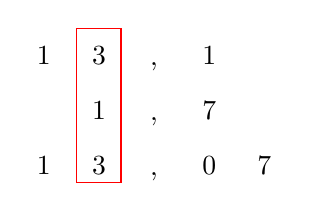
\begin{tikzpicture}[scale=0.7]
                \draw (0,0) node {1} ;
                \draw (1,0) node {3} ; 
                \draw (2,-0.2) node {,} ;
                \draw (3,0) node {1} ;
                \draw (1,-1) node {1} ; 
                \draw (2,-1.2) node {,} ;
                \draw (3,-1) node {7} ;
                \draw (0,-2) node {1} ;
                \draw (1,-2) node {3} ;
                \draw (2,-2.2) node {,} ;
                \draw (3,-2) node {0} ;
                \draw (4,-2) node {7} ;
                \draw [red] (0.6,0.5) rectangle (1.4,-2.3);
            \end{tikzpicture}
        }
    \end{figure}
\end{minipage}
\begin{minipage}{0.7\textwidth}    
    On complête avec des 0 à droite et à gauche pour que tous les nombres aient autant de chiffres. 
\end{minipage}
\hfill
\begin{minipage}{0.22\textwidth}
    \begin{figure}[H]
    \centering
        \resizebox{\textwidth}{!}{
            \begin{tikzpicture}[scale=0.7]
                \draw (0,0) node {1} ;
                \draw (1,0) node {3} ; 
                \draw (2,-0.2) node {,} ;
                \draw (3,0) node {1} ;
                \draw [red] (4,0) node {0} ;
                \draw [red] (0,-1) node {0} ;
                \draw (1,-1) node {1} ; 
                \draw (2,-1.2) node {,} ;
                \draw (3,-1) node {7} ;
                \draw [red] (4,-1) node {0} ;
                \draw (0,-2) node {1} ;
                \draw (1,-2) node {3} ;
                \draw (2,-2.2) node {,} ;
                \draw (3,-2) node {0} ;
                \draw (4,-2) node {7} ;
            \end{tikzpicture}
        }
    \end{figure}
\end{minipage}
\begin{minipage}{0.7\textwidth}    
    Le nombre le plus sera celui avec le chiffre de gauche le plus petit. Ici c'est le 0 de 01,70.  C'est donc 1,7 .
\end{minipage}
\hfill
\begin{minipage}{0.22\textwidth}
    \begin{figure}[H]
    \centering
        \resizebox{\textwidth}{!}{
            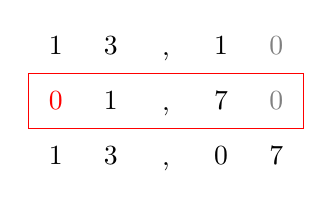
\begin{tikzpicture}[scale=0.7]
                \draw (0,0) node {1} ;
                \draw (1,0) node {3} ; 
                \draw (2,-0.2) node {,} ;
                \draw (3,0) node {1} ;
                \draw [gray] (4,0) node {0} ;
                \draw [red] (0,-1) node {0} ;
                \draw (1,-1) node {1} ; 
                \draw (2,-1.2) node {,} ;
                \draw (3,-1) node {7} ;
                \draw [gray] (4,-1) node {0} ;
                \draw (0,-2) node {1} ;
                \draw (1,-2) node {3} ;
                \draw (2,-2.2) node {,} ;
                \draw (3,-2) node {0} ;
                \draw (4,-2) node {7} ;
                \draw [red] (-0.5,-0.5) rectangle (4.5,-1.5);
            \end{tikzpicture}
        }
    \end{figure}
\end{minipage}
\begin{minipage}{0.7\textwidth}    
    On recommence ensuite avec les nombres restant. Si deux nombres commencent avec le même chiffre, on prend le chiffre suivant.
\end{minipage}
\hfill
\begin{minipage}{0.22\textwidth}
    \begin{figure}[H]
    \centering
        \resizebox{\textwidth}{!}{
            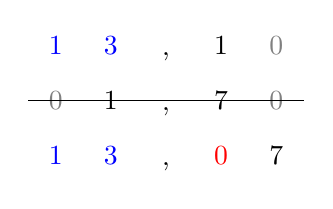
\begin{tikzpicture}[scale=0.7]
                \draw [blue] (0,0) node {1} ;
                \draw [blue] (1,0) node {3} ; 
                \draw (2,-0.2) node {,} ;
                \draw (3,0) node {1} ;
                \draw [gray] (4,0) node {0} ;
                \draw [gray] (0,-1) node {0} ;
                \draw (1,-1) node {1} ; 
                \draw (2,-1.2) node {,} ;
                \draw (3,-1) node {7} ;
                \draw [gray] (4,-1) node {0} ;
                \draw [blue] (0,-2) node {1} ;
                \draw [blue] (1,-2) node {3} ;
                \draw (2,-2.2) node {,} ;
                \draw [red] (3,-2) node {0} ;
                \draw (4,-2) node {7} ;
                \draw (-0.5,-1) -- (4.5,-1) ;[blue] 
            \end{tikzpicture}
        }
    \end{figure}
\end{minipage}\\
Le deuxième nombre est ici 13,07. Le dernier est donc 13,1. \\
L'ordre croissant est donc 1,7 ; 13,07 ; 13,1.
}